\chapter{Měření}

V této kapitole stručně představíme výsledky měření, detailní grafy ke každému pozorovateli zvlášť jsou v první příloze této práce.

\section{Výsledky}
\begin{figure}[h!]
\centering
\begin{tabular}{c}
\begin{subfigure}{0.80\textwidth}
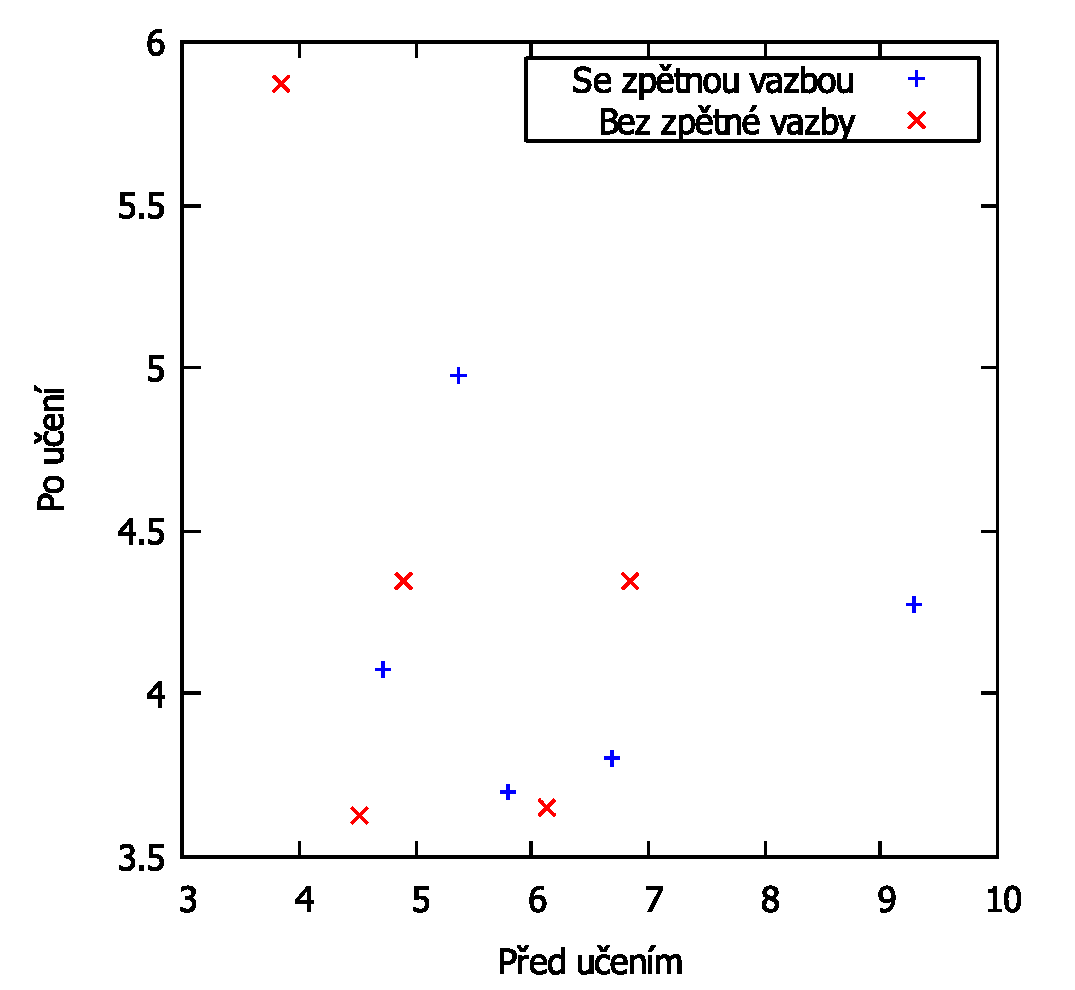
\includegraphics[width=0.99\linewidth]{graphs/AverageTries}
\caption{Průměrný počet fixací}
\end{subfigure}\\
\end{tabular}
\end{figure}
\begin{figure}[h!]
\begin{tabular}{c}
\begin{subfigure}{0.80\textwidth}
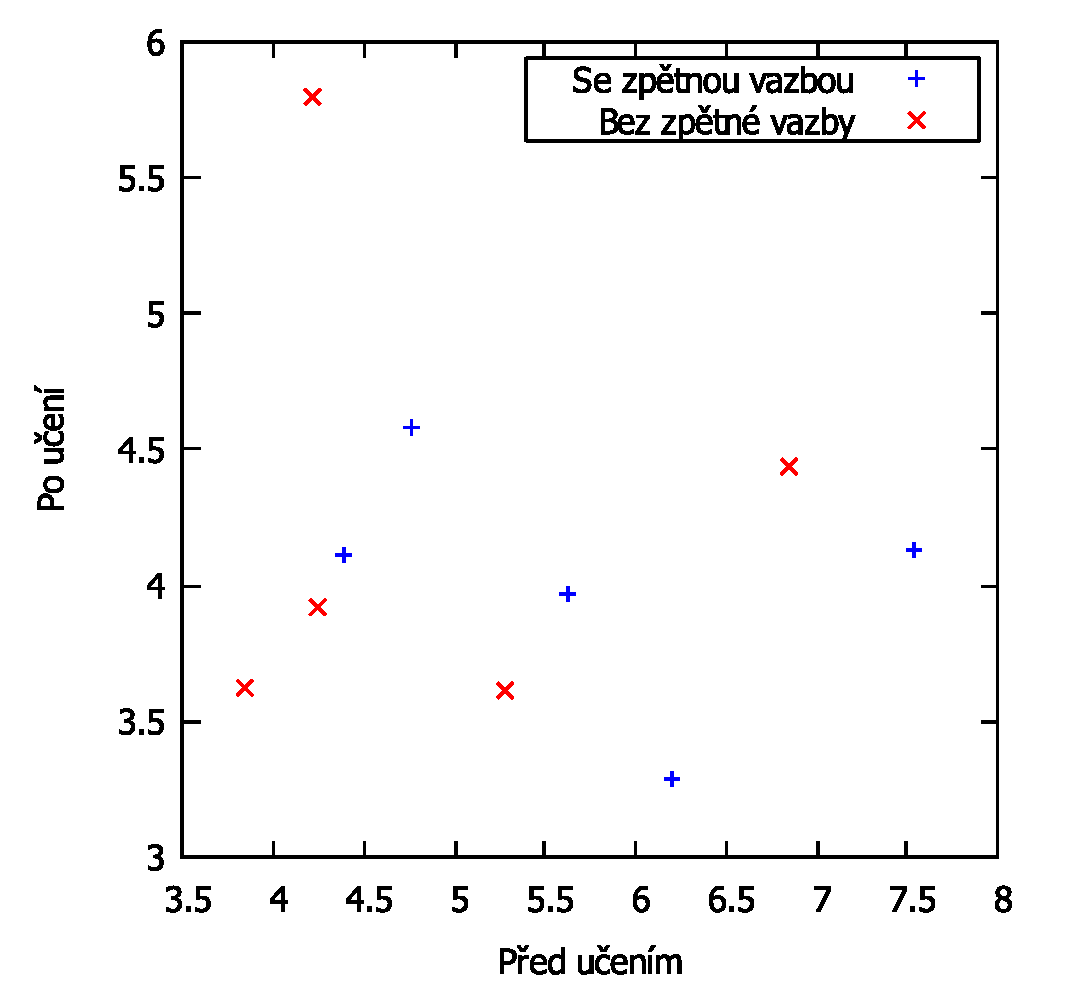
\includegraphics[width=0.99\linewidth]{graphs/AverageSuccesfullTries}
\caption{Průměrný počet fixací v úspěšně splněných úkolech}
\end{subfigure}\\

\begin{subfigure}{0.80\textwidth}
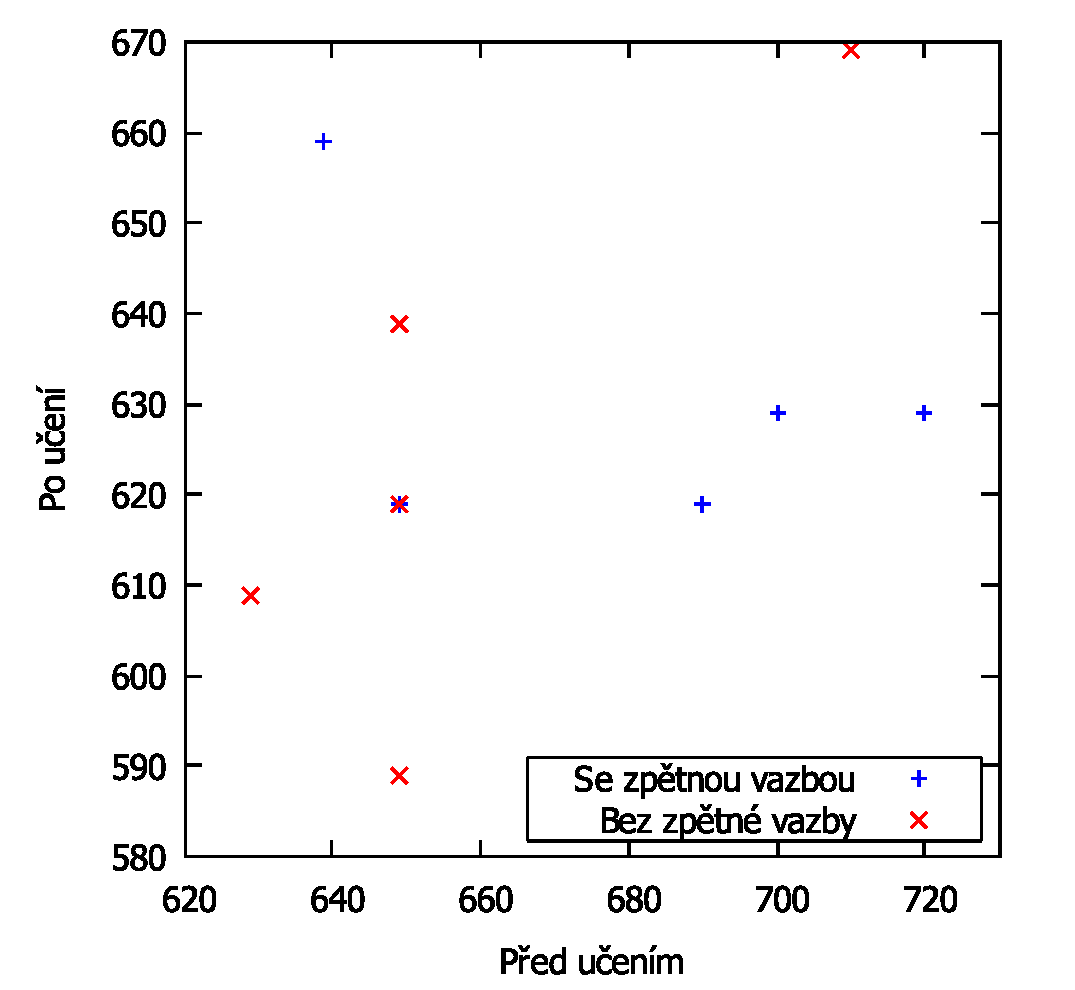
\includegraphics[width=0.99\linewidth]{graphs/FinalDifficulty}
\caption{Obtížnost po 40. pokusu}
\end{subfigure}\\


\end{tabular}
\end{figure}
